\documentclass[border={1cm 1cm 1cm 0.5cm}]{standalone}

\usepackage{tikz}
\usetikzlibrary{calc}					%for centerarc
\usetikzlibrary{shadings}				%for diagonal shading
\usetikzlibrary{shapes.geometric}		%for hexagons, cylinders
\usetikzlibrary{shapes.symbols}			%for clouds

\def\centerarc[#1](#2)(#3:#4:#5)% Syntax: [draw options] (center) (initial angle:final angle:radius)
{ \draw[#1] ($(#2)+({#5*cos(#3)},{#5*sin(#3)})$) arc (#3:#4:#5); }

%``Cryometric Index of Poetic Forms,'' from Bök - Crystallography (2003), p. 115

\begin{document}
	
	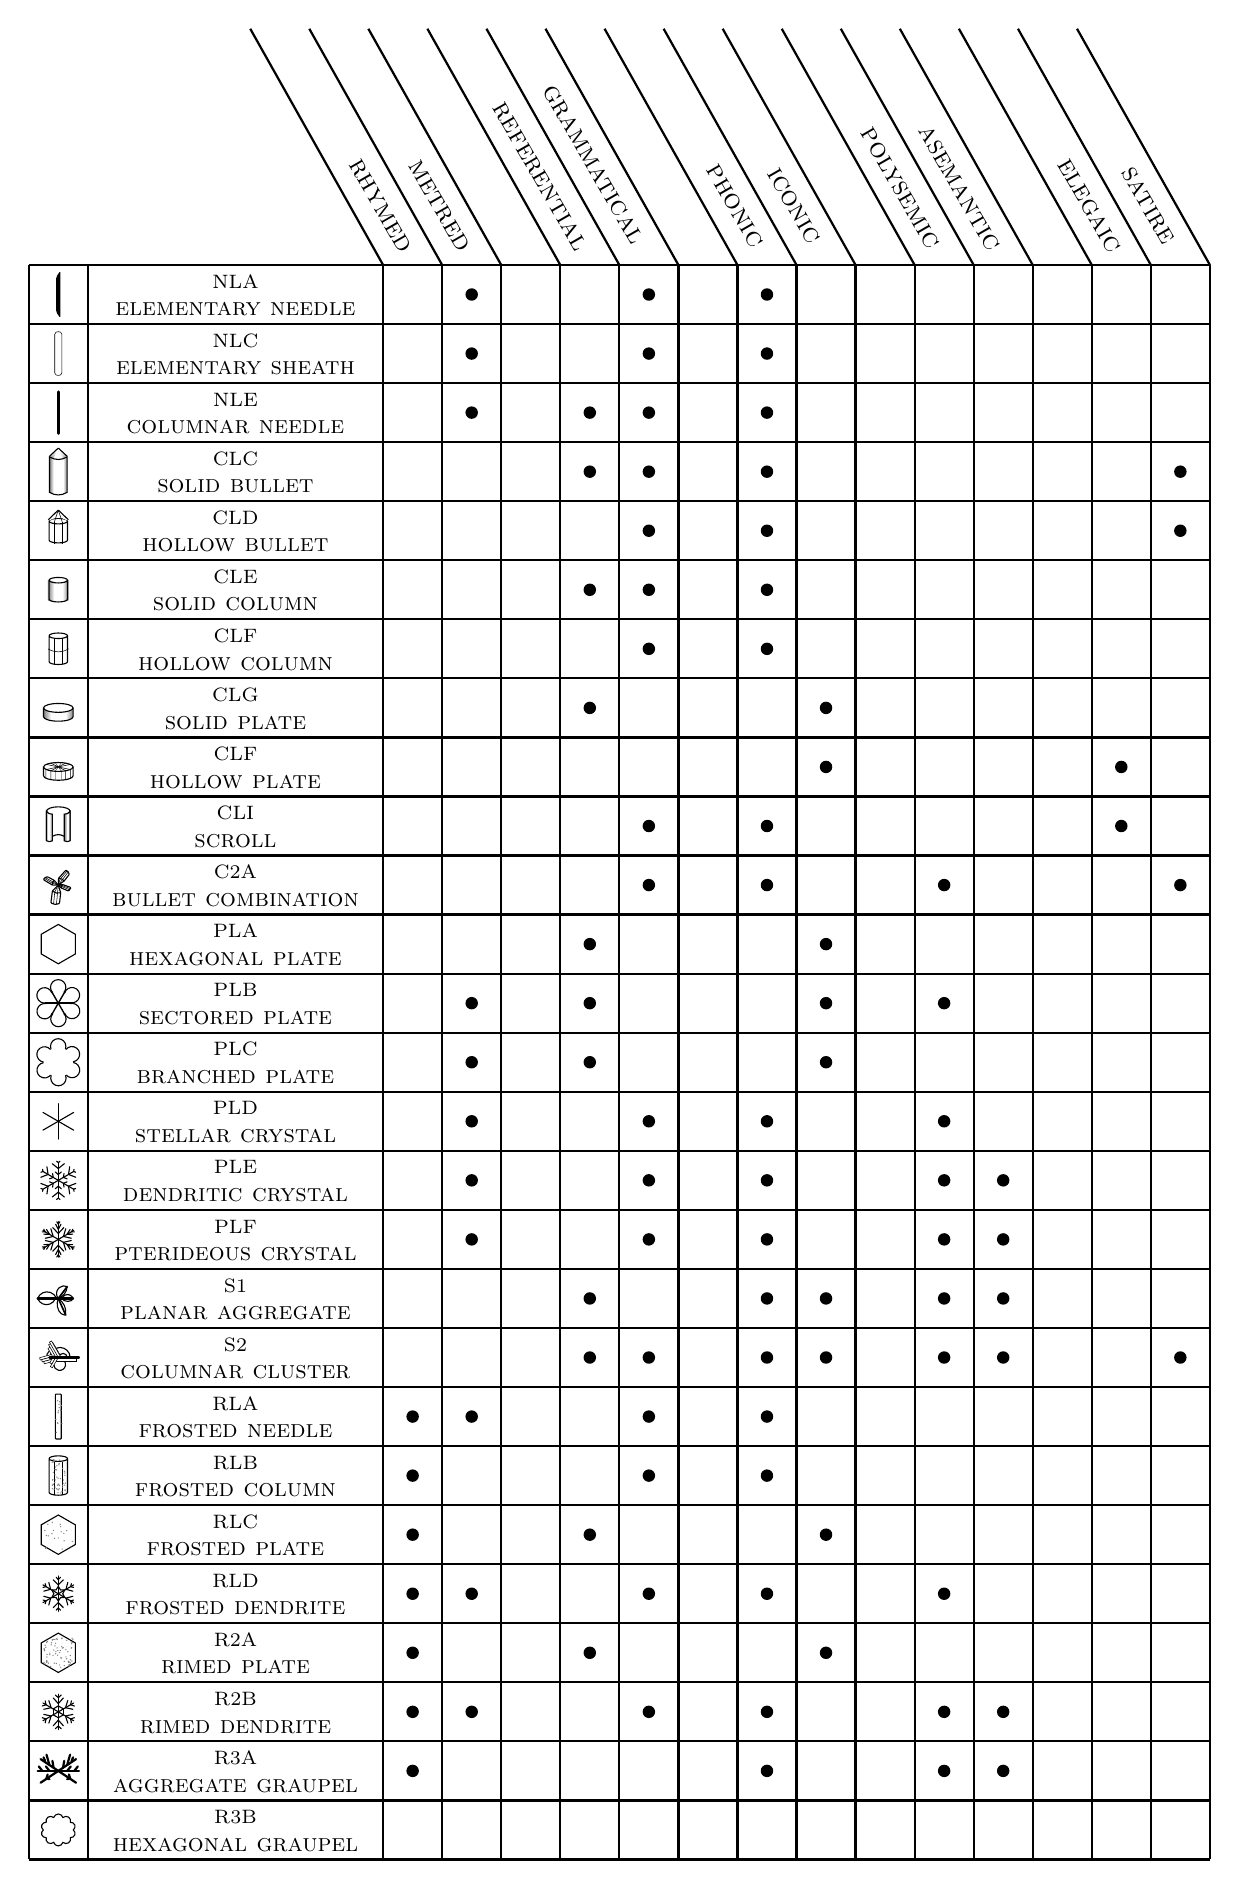
\begin{tikzpicture}[scale=0.75]
	%TABLE
	\foreach \x in {0,...,14} \draw[thick] (5.5+\x,26.5)--(3.25+\x,30.5);	%diagonals
	\draw[thick,xshift=-0.5cm,yshift=-0.5cm] (0,0) grid (1,27);			 	%leftmost column
	\foreach \x in {0,...,27} \draw[thick] (0.5,-0.5+\x)--(5.5,-0.5+\x); 	%wide column
	\draw[thick,xshift=-0.5cm,yshift=-0.5cm] (6,0) grid (20,27);		 	%rightward grid
	
	%DOTS
	\foreach \x in {1,...,7} \fill (6,\x) circle (3pt);	%first column
	\foreach \x in {3,5,8,11,12,13,14,15,25,26,27} \fill (7,\x-1) circle (3pt); %second
	\foreach \x in {4,6,9,10,14,15,16,20,22,24,25} \fill (9,\x-1) circle (3pt); %fourth
	\foreach \x in {3,5,7,8,9,11,12,13,17,18,21,22,23,24,25,26,27} \fill (10,\x-1) circle (3pt); %5
	\foreach \x in {2,3,5,7,8,9,10,11,12,13,17,18,21,22,23,24,25,26,27} \fill (12,\x-1) circle (3pt); %7
	\foreach \x in {4,6,9,10,14,15,16,19,20} \fill (13,\x-1) circle (3pt); %8
	\foreach \x in {2,3,5,9,10,11,12,13,15,17} \fill (15,\x-1) circle (3pt); %10
	\foreach \x in {2,3,9,10,11,12} \fill (16,\x-1) circle (3pt); %11
	\foreach \x in {18,19} \fill (18,\x-1) circle (3pt); %13
	\foreach \x in {9,17,23,24} \fill (19,\x-1) circle (3pt); %14
	
	%DIAGONAL LABELS
	\node at (5.45,27.5) {\rotatebox{-60}{\textsc{rhymed}}};
	\node at (6.45,27.5) {\rotatebox{-60}{\textsc{metred}}};
	\node at (8.15,28) {\rotatebox{-60}{\textsc{referential}}};
	\node at (9.05,28.2) {\rotatebox{-60}{\textsc{grammatical}}};
	\node at (11.45,27.5) {\rotatebox{-60}{\textsc{phonic}}};
	\node at (12.45,27.5) {\rotatebox{-60}{\textsc{iconic}}};
	\node at (14.25,27.8) {\rotatebox{-60}{\textsc{polysemic}}};
	\node at (15.25,27.8) {\rotatebox{-60}{\textsc{asemantic}}};
	\node at (17.45,27.5) {\rotatebox{-60}{\textsc{elegaic}}};
	\node at (18.45,27.5) {\rotatebox{-60}{\textsc{satire}}};
	
	%LABELS
	\node at (3,25.75) {\small\textsc{elementary needle}};	\node at (3,26.22) {\scriptsize NLA};
	\node at (3,24.75) {\small\textsc{elementary sheath}};	\node at (3,25.22) {\scriptsize NLC};
	\node at (3,23.75) {\small\textsc{columnar needle}};	\node at (3,24.22) {\scriptsize NLE};
	\node at (3,22.75) {\small\textsc{solid bullet}};		\node at (3,23.22) {\scriptsize CLC};
	\node at (3,21.75) {\small\textsc{hollow bullet}};		\node at (3,22.22) {\scriptsize CLD};
	\node at (3,20.75) {\small\textsc{solid column}};		\node at (3,21.22) {\scriptsize CLE};
	\node at (3,19.75) {\small\textsc{hollow column}};		\node at (3,20.22) {\scriptsize CLF};
	\node at (3,18.75) {\small\textsc{solid plate}};		\node at (3,19.22) {\scriptsize CLG};
	\node at (3,17.75) {\small\textsc{hollow plate}};		\node at (3,18.22) {\scriptsize CLF};
	\node at (3,16.75) {\small\textsc{scroll}};				\node at (3,17.22) {\scriptsize CLI};
	\node at (3,15.75) {\small\textsc{bullet combination}};	\node at (3,16.22) {\scriptsize C2A};
	\node at (3,14.75) {\small\textsc{hexagonal plate}};	\node at (3,15.22) {\scriptsize PLA};
	\node at (3,13.75) {\small\textsc{sectored plate}};		\node at (3,14.22) {\scriptsize PLB};
	\node at (3,12.75) {\small\textsc{branched plate}};		\node at (3,13.22) {\scriptsize PLC};
	\node at (3,11.75) {\small\textsc{stellar crystal}};	\node at (3,12.22) {\scriptsize PLD};
	\node at (3,10.75) {\small\textsc{dendritic crystal}};	\node at (3,11.22) {\scriptsize PLE};
	\node at (3, 9.75) {\small\textsc{pterideous crystal}};	\node at (3,10.22) {\scriptsize PLF};
	\node at (3, 8.75) {\small\textsc{planar aggregate}};	\node at (3, 9.22) {\scriptsize S1};
	\node at (3, 7.75) {\small\textsc{columnar cluster}};	\node at (3, 8.22) {\scriptsize S2};
	\node at (3, 6.75) {\small\textsc{frosted needle}};		\node at (3, 7.22) {\scriptsize RLA};
	\node at (3, 5.75) {\small\textsc{frosted column}};		\node at (3, 6.22) {\scriptsize RLB};
	\node at (3, 4.75) {\small\textsc{frosted plate}};		\node at (3, 5.22) {\scriptsize RLC};
	\node at (3, 3.75) {\small\textsc{frosted dendrite}};	\node at (3, 4.22) {\scriptsize RLD};
	\node at (3, 2.75) {\small\textsc{rimed plate}};		\node at (3, 3.22) {\scriptsize R2A};
	\node at (3, 1.75) {\small\textsc{rimed dendrite}};		\node at (3, 2.22) {\scriptsize R2B};
	\node at (3, 0.75) {\small\textsc{aggregate graupel}};	\node at (3, 1.22) {\scriptsize R3A};
	\node at (3,-0.25) {\small\textsc{hexagonal graupel}};	\node at (3, 0.22) {\scriptsize R3B};
	
	%CRYSTALS
	%elementary needle
	\fill[rounded corners=0.5pt] (0-0.07/2,26-0.25)--++(0,0.55)--++(0.07,0.1)--++(0,-0.8)--++(-0.07,0.1)--cycle;
	
	%elementary sheath
	\filldraw[fill=white,draw=black,very thin,rounded corners=0.5pt] (0-0.12/2,25-0.35)--++(0,2*0.35) to[bend left] ++(0.12,0) -- ++(0,-2*0.35) to[bend left] ++(-0.12,0) -- cycle;
	
	%columnar needle
	\draw[very thick,line cap=round] (0,24-0.35)--++(0,0.7);
	
	%solid bullet
	%shading, left rectangle
	\shade[left color=gray,right color=white] (-0.08,23-0.39)--(-0.15,23-0.35)--(-0.15,23+0.26)--(-0.08,23+0.225)--(-0.15,23+0.26)--(-0.08,23+0.225)--cycle;
	%shading, left triangle
	\shade[lower left=gray,upper right=white] (-0.15,23+0.26)--(0,23+0.4)--(-0.08,23+0.225)--cycle;
	%shading, right rectangle
	\shade[left color=white,right color=gray] (.08,23-0.39)--(.15,23-0.35)--(.15,23+0.26)--(.08,23+0.225)--(.15,23+0.26)--(.08,23+.225)--cycle;
	%shading, right triangle
	\shade[lower right=gray,upper left=white] (0.15,23+0.26)--(0,23+0.4)--(0.08,23+0.225)--cycle;
	%
	\draw[rounded corners=0.25pt] (-0.15,23+0.26)--(0,23+0.4)--(0.15,23+0.26);		%point, top
	\draw (-0.15,23-0.35)--(-0.15,23+0.25) to[bend right] (0.15,23+0.25) -- 
	(0.15,23-0.35) to[bend left] (-0.15,23-0.35)--cycle;
	%borders, not needed with shading
	%	\draw[very thin, rounded corners=0.25pt] (-0.08,23+0.225)--(0,23+0.4)--(0.08,23+0.225);	%point, low
	%	\draw[very thin] (-0.08,23-0.39)--(-0.08,23+0.225);	%vertical line, left
	%	\draw[very thin] ( 0.08,23-0.39)--( 0.08,23+0.225);	%vertical line, right
	
	%hollow bullet
	\node[cylinder,draw,shape border rotate=90,shape aspect=.3] at (0,22-0.05) {};
	\draw[white,line width=0.7pt] (-0.16,22+0.189) to[bend left] (0.16,22+0.189);
	\draw[rounded corners=0.25pt] (-0.17,22+0.186)--(0,22+0.35)--(0.17,22+0.186);	%point, top
	\draw[very thin,rounded corners=0.25pt] (-0.07,22+0.14)--(0,22+0.35)--(0.07,22+0.14); %point, low
	\draw[very thin] (-0.07,22-0.22)--(-0.07,22+0.14);		%left vertical line
	\draw[very thin] ( 0.07,22-0.22)--( 0.07,22+0.14);		%right vertical line
	
	%solid column
	\shade[left color=gray,right color=white] (-0.07,21-0.22)--(-0.175,21-0.18)--(-0.175,21+0.17)--(-0.07,21+0.14)--cycle; %L
	\shade[left color=white,right color=gray] (0.07,21-0.22)--(0.175,21-0.18)--(0.175,21+0.17)--(0.07,21+0.14)--cycle; %R
	\node[cylinder,draw,shape border rotate=90,shape aspect=.3] at (0,21-0.05) {};
	%
	%	\draw[very thin,gray!70] (-0.07,21-0.22)--(-0.07,21+0.14);	%vertical line, left
	%	\draw[very thin,gray!70] ( 0.07,21-0.22)--( 0.07,21+0.14);	%vertical line, right
	
	%hollow column
	\node[cylinder,draw,shape border rotate=90,shape aspect=.3,minimum height=0.4cm] at (0,20-0.05) {};
	\draw[very thin] (-0.175,20-0) to[bend right] (0.175,20-0);
	\draw[very thin] (-0.07,20-0.25)--(-0.07,20+0.18);	%vertical line, left
	\draw[very thin] ( 0.07,20-0.25)--( 0.07,20+0.18);	%vertical line, right
	
	%solid plate
	\shade[left color=gray,right color=white] (-0.25,19-0)--(-0.25,19-0.15) arc (180:240:0.25 and 0.075) -- ++(0,0.15) arc (-120:-175:0.25 and 0.075) -- cycle;	%shading left
	\shade[left color=white,right color=gray] (0.125,19-0.065)--(0.125,19-0.215) arc (300:360:0.25 and 0.075) -- ++(0,0.145) arc (-5:-60:0.25 and 0.075) -- cycle;	%shading right
	\draw (0,19) ellipse (0.25 and 0.075);
	\draw (-0.25,19-0)--(-0.25,19-0.15) arc (180:360:0.25 and 0.075) --(0.25,19-0);
	
	%hollow plate
	\draw (0,18) ellipse (0.25 and 0.075);
	\draw (-0.25,18-0)--(-0.25,18-0.15) arc (180:360:0.25 and 0.075) --(0.25,18-0);
	\draw[very thin] (0,18-0)--(-0.125,18+0.065);
	\draw[very thin] (0,18-0)--( 0.125,18+0.065);
	\draw[very thin] (-0.125,18-0.215)--(-0.125,18-0.065)--(0,18-0);
	\draw[very thin] ( 0.125,18-0.215)--( 0.125,18-0.065)--(0,18-0);
	%
	\draw[ultra thin] (0,18-0)--(-0.05,18+0.07);	%innermost vertical lines
	\draw[ultra thin] (0,18-0)--( 0.05,18+0.07);
	\draw[ultra thin] (-0.05,18-0.22)--(-0.05,18-0.07)--(0,18-0);
	\draw[ultra thin] ( 0.05,18-0.22)--( 0.05,18-0.07)--(0,18-0);
	%
	\draw[very thin] (0,18-0)--(-0.21,18+0.045);
	\draw[very thin] (0,18-0)--( 0.21,18+0.045);
	\draw[very thin] (-0.21,18-0.2)--(-0.21,18-0.045)--(0,18-0);
	\draw[very thin] ( 0.21,18-0.2)--( 0.21,18-0.045)--(0,18-0);
	
	%scroll
	\shade[left color=white,right color=gray] %shade left
	(-.1,17+0.2)--(-.15,17+0.22)--(-.15,17-0.27)--(-.1,17-0.25)--cycle;
	\shade[left color=gray,right color=white] %shade right
	(0.1,17+0.2)--(0.15,17+0.22)--(0.15,17-0.27)--(0.1,17-0.25)--cycle;
	\draw (-0.2,17-0.25)--(-0.2,17+0.25) arc (180:0:0.2 and 0.075) -- (0.2,17-0.25);
	\draw (-.2,17+0.25) to[bend right] (-.1,17+0.2)--(-.1,17-0.25) to[bend left] (-.2,17-0.25)--cycle;
	\draw (0.2,17+0.25) to[bend left] (0.1,17+0.2)--(0.1,17-0.25) to[bend right] (0.2,17-0.25)--cycle;	
	\draw (-0.1,17-0.175) to[bend left] (0.1,17-0.175); %bottom bend in center
	
	%bullet combination
	%several hollow columns rotated at various degrees and joined by points at the origin
%	\draw[step=.125cm, help lines] (-0.5,15.5) grid (0.5,16.5);
%	\fill[blue] (0,16) circle (0.5pt);
	%bottom
	\draw[rounded corners=0.25pt] (0,16)--(-0.1,16-0.1)--(-0.125,16-0.3) to[bend right] (0.02,16-0.31) -- (0.04,16-0.13)--cycle;
	\draw (-0.1,16-0.1) to[bend right] (0.04,16-0.13);
	\draw[very thin] (0,16)--(-0.06,16-0.115)--(-0.08,16-0.32);	%left
	\draw[very thin] (0,16)--(-0.0313,16-0.323);	%right
	%
	%leftmost
	\draw[rounded corners=0.25pt] (0,16)--(-0.1,16)--(-0.25,16+0.09) to[bend left] (-0.18,16+0.14) --(-0.07,16+0.08)--cycle;
	\draw (-0.1,16) to[bend left] (-0.07,16+0.08);
	\draw[very thin] (0,16)--(-0.215,16+0.125);	%right
	\draw[very thin] (0,16)--(-0.1,16+0.03)--(-0.23,16+0.11);	%left
	%
	%top
	\draw[rounded corners=0.25pt] (0,16)--(0,16+0.11)--(0.125,16+0.25) to[bend left] (0.185,16+0.18)--(0.1,16+0.07)--cycle;
	\draw (0,16+0.11) to[bend left] (0.1,16+0.07);
	\draw[very thin] (0,16)--(0.03,16+0.1)--(0.15,16+0.24);
	\draw[very thin] (0,16)--(0.17,16+0.225);
	%
	%right
	\draw[rounded corners=0.25pt] (0,16)--(0.07,16+0.01)--(0.21,16-0.04) to[bend left] (0.17,16-0.1)--(0.05,16-0.05)--cycle;
	\draw (0.07,16+0.01) to[bend left] (0.05,16-0.05);
	\draw[very thin] (0,16)--(0.07,16-0.01)--(0.2,16-0.06);
	\draw[very thin] (0,16)--(0.19,16-0.08);
	
	%hexagonal plate
	\node[regular polygon,regular polygon sides=6,minimum size=0.5cm,draw,rotate=30] at (0,15) {};
	
	%sectored plate
	%\draw[ultra thin,red] (0,14) circle (0.2);
	%\draw[ultra thin,red] (0,14) circle (0.4);
	\foreach \x in {0,...,5}{
	\draw ({0.2*cos(90+28+60*\x)},{14+0.2*sin(90+28+60*\x)}) arc (180+45+60*\x:0-42+60*\x:0.13cm);
	\draw[line width=0.5] ({0.22*cos(90+30+60*\x)},{14+0.22*sin(90+30+60*\x)}) -- (0,14);
		}	%end of loop
	
	%branched plate
	\foreach \x in {0,...,5} 
	\draw ({0.2*cos(90+28+60*\x)},{13+0.2*sin(90+28+60*\x)}) arc (180+45+60*\x:0-42+60*\x:0.13cm);
	\fill[white] (0,13) circle (0.25);
	
	%stellar crystal
	\foreach \x in {0,...,5} 
	\draw[line cap=round] (0,12)--++({0.3*cos(90+60*\x)},{0.3*sin(90+60*\x)});
	
	%dendritic crystal
	\foreach \x in {0,...,5}{
	\draw[line cap=round] (0,11)--++({0.3*cos(90+60*\x)},{0.3*sin(90+60*\x)});
	\draw[line cap=round] %closest to center, left (90+20)
	({0.1*cos(90+60*\x)},{11+0.1*sin(90+60*\x)})--({0.15*cos(110+60*\x)},{11+0.15*sin(110+60*\x)});
	\draw[line cap=round] %closest to center, right (90-20)
	({0.1*cos(90+60*\x)},{11+0.1*sin(90+60*\x)})--({0.15*cos(70+60*\x)},{11+0.15*sin(70+60*\x)});
	\draw[line cap=round] %middle, longest, left
	({0.2*cos(90+60*\x)},{11+0.2*sin(90+60*\x)})--({0.3*cos(110+60*\x)},{11+0.3*sin(110+60*\x)});
	\draw[line cap=round] %middle, longest, right
	({0.2*cos(90+60*\x)},{11+0.2*sin(90+60*\x)})--({0.3*cos(70+60*\x)},{11+0.3*sin(70+60*\x)});
	\draw[line cap=round] %tip of snowflake left
	({0.3*cos(90+60*\x)},{11+0.3*sin(90+60*\x)})--({0.325*cos(95+60*\x)},{11+0.325*sin(95+60*\x)});
	\draw[line cap=round] %tip of snowflake, right
	({0.3*cos(90+60*\x)},{11+0.3*sin(90+60*\x)})--({0.325*cos(85+60*\x)},{11+0.325*sin(85+60*\x)});
		} %end of loop
	
	%pterideous crystal
	\foreach \x in {0,...,5}{
	\draw[line cap=round] (0,10)--++({0.3*cos(90+60*\x)},{0.3*sin(90+60*\x)});
	\draw[line cap=round] %closest to center, left (90+20)
	({0.1*cos(90+60*\x)},{10+0.1*sin(90+60*\x)})--({0.22*cos(115+60*\x)},{10+0.22*sin(115+60*\x)});
	\draw[line cap=round] %closest to center, right (90-20)
	({0.1*cos(90+60*\x)},{10+0.1*sin(90+60*\x)})--({0.22*cos(65+60*\x)},{10+0.22*sin(65+60*\x)});
	\draw[line cap=round] %middle, longest, left
	({0.17*cos(90+60*\x)},{10+0.17*sin(90+60*\x)})--({0.26*cos(100+60*\x)},{10+0.26*sin(100+60*\x)});
	\draw[line cap=round] %middle, longest, right
	({0.17*cos(90+60*\x)},{10+0.17*sin(90+60*\x)})--({0.26*cos(80+60*\x)},{10+0.26*sin(80+60*\x)});
	\draw[line cap=round] %tip of snowflake left
	({0.26*cos(90+60*\x)},{10+0.26*sin(90+60*\x)})--({0.3*cos(95+60*\x)},{10+0.3*sin(95+60*\x)});
	\draw[line cap=round] %tip of snowflake, right
	({0.26*cos(90+60*\x)},{10+0.26*sin(90+60*\x)})--({0.3*cos(85+60*\x)},{10+0.3*sin(85+60*\x)});
		} %end of loop
	
	%planar aggregate
	\draw[thick,line cap=round] (-0.35,9)--(0.25,9);
		\draw[semithick,line cap=round] (0,9)--(0.15,9+0.2);	%0--NE
		\draw[semithick,line cap=round] (0,9)--(0.125,9-0.28);	%0--SE
	\draw (-0.35,9) arc (180-20:0+20:0.17cm);		%left petal,top
	\draw (-0.35,9) arc (180+20:360-20:0.16cm);		%left petal,bottom
	\draw (0.25,9) arc (0+20:180-20:0.1cm);			%right petal,top
	\draw (0.25,9) arc (360:180:0.09cm and 0.05cm);	%right petal,bottom
	\draw (0,9) arc (220:65:0.13cm);				%NE petal, left
	\draw (0,9) to[bend right] (0.15,9+0.2);		%NE petal, right
	\draw (0,9) arc (150:270:0.14cm and 0.19cm);	%SE petal, left
	\draw (0,9) to[bend left] (0.125,9-0.28);		%SE petal, right
	
	%columnar cluster
	\draw (0.2,8) arc (0:180:0.17cm);		%top big arc
	\draw (0.15,8) arc (0:180:0.07cm);		%top little arc
	\draw (0.04,8-.02) arc (80:-180:0.1cm);	%bottom arc
	\draw (-0.2,8) arc (180:90:0.15cm);		%leftmost arc
	%
	\filldraw[fill=white,draw=black,very thin] (-0.1,8-0.02) rectangle (0.3,8-0.06); %horizontal
	%
	\filldraw[fill=white,draw=black,very thin,rotate around={15:(-0.08,8+0.06)}] (-0.08,8+0.06) rectangle (-0.325,8+0.02);	%leftmost bars
	\filldraw[fill=white,draw=black,very thin,rotate around={15:(-0.08,8+0.06)}] (-0.08,8+0.02) rectangle (-0.3,8-0.02);
	\filldraw[fill=white,draw=black,very thin,rotate around={15:(-0.08,8+0.06)}] (-0.08,8-0.02) rectangle (-0.275,8-0.06);
	%
	\filldraw[fill=white,draw=black,very thin,rotate around={30:(-0.04,8)}] (-0.08,8.01) rectangle (0.04,8+0.2); %upper bars, shortest
	\filldraw[fill=white,draw=black,very thin,rotate around={30:(-0.04,8)}] (-0.04,8) rectangle (0.04,8+0.25);
	\filldraw[fill=white,draw=black,very thin,rotate around={30:(0,8)}] (0,8) rectangle (0.04,8+0.3); %longest
	%
	\filldraw[fill=white,draw=black,very thin,rotate around={150:(0,8)}] (0,8.01) rectangle (0.04,8+0.2); %lower bars, longest
	\filldraw[fill=white,draw=black,very thin,rotate around={150:(0,8)}] (0.08,8.01) rectangle (0.04,8+0.15);
	%
	\draw[thick,line cap=round] (-0.15,8)--(0.35,8);	%horizontal line
	
	%frosted needle
	\draw[rounded corners=0.25pt] (0-0.05,7-0.38) rectangle (0+0.05,7+0.38);
	\foreach \p in {1,...,15} \fill[gray] (0.075*rand,7+0.32*rand) circle (0.35pt); %random dots
	%\draw[very thin, red] (0,7) ellipse (0.075 and 0.32);
	
	%frosted column
	\node[cylinder,draw,shape border rotate=90,shape aspect=.3,minimum height=0.5cm] at (0,6-0.05) {};
	\draw[very thin] (-0.07,6-0.33)--(-0.07,6+0.23);
	\draw[very thin] ( 0.07,6-0.33)--( 0.07,6+0.23);
	\foreach \p in {1,...,50} \fill[gray] (0.12*rand,6+0.3*rand) circle (0.35pt); %random dots
	%\draw[very thin, red] (0,6) ellipse (0.12 and 0.3);
	
	%frosted plate
	\node[regular polygon,regular polygon sides=6,minimum size=0.5cm,draw,rotate=30] at (0,5) {};
	\foreach \p in {1,...,20} \fill[gray] (0.25*rand,5+0.25*rand) circle (0.35pt); %random dots
	%\draw[very thin,red] (0,5) circle (0.25cm);
	
	%frosted dendrite
	\foreach \x in {0,...,5}{
	\draw[line cap=round] (0,4)--++({0.3*cos(90+60*\x)},{0.3*sin(90+60*\x)});
	\draw[line cap=round] %closest to center, left (90+20)
	({0.125*cos(90+60*\x)},{4+0.125*sin(90+60*\x)})--({0.075*cos(120+60*\x)},{4+0.075*sin(120+60*\x)});
	\draw[line cap=round] %closest to center, right (90-20)
	({0.125*cos(90+60*\x)},{4+0.125*sin(90+60*\x)})--({0.075*cos(60+60*\x)},{4+0.075*sin(60+60*\x)});
	\draw[line cap=round] %middle, longest, left
	({0.15*cos(90+60*\x)},{4+0.15*sin(90+60*\x)})--({0.25*cos(110+60*\x)},{4+0.25*sin(110+60*\x)});
	\draw[line cap=round] %middle, longest, right
	({0.15*cos(90+60*\x)},{4+0.15*sin(90+60*\x)})--({0.25*cos(70+60*\x)},{4+0.25*sin(70+60*\x)});
	\draw[line cap=round] %furthest branch, left
	({0.24*cos(90+60*\x)},{4+0.24*sin(90+60*\x)})--({0.28*cos(97.5+60*\x)},{4+0.28*sin(97.5+60*\x)});
	\draw[line cap=round] %furthest branch, right
	({0.24*cos(90+60*\x)},{4+0.24*sin(90+60*\x)})--({0.28*cos(82.5+60*\x)},{4+0.28*sin(82.5+60*\x)});
	} %end of loop
	
	%rimed plate
	\node[regular polygon,regular polygon sides=6,minimum size=0.5cm,draw,rotate=30] at (0,3) {};
	\foreach \p in {1,...,75} \fill[gray] (0.25*rand,3+0.25*rand) circle (0.35pt); %random dots
	
	%rimed dendrite
	\foreach \x in {0,...,5}{
	\draw[line cap=round] (0,2)--++({0.3*cos(90+60*\x)},{0.3*sin(90+60*\x)});
	\draw[line cap=round] %hexagon in center
	({0.1*cos(90+60*\x)},{2+0.1*sin(90+60*\x)})--({0.1*cos(150+60*\x)},{2+0.1*sin(150+60*\x)});
	\draw[line cap=round] %middle, longest, left
	({0.14*cos(90+60*\x)},{2+0.14*sin(90+60*\x)})--({0.25*cos(110+60*\x)},{2+0.25*sin(110+60*\x)});
	\draw[line cap=round] %middle, longest, right
	({0.14*cos(90+60*\x)},{2+0.14*sin(90+60*\x)})--({0.25*cos(70+60*\x)},{2+0.25*sin(70+60*\x)});
	\draw[line cap=round] %furthest branch, left
	({0.24*cos(90+60*\x)},{2+0.24*sin(90+60*\x)})--({0.29*cos(100+60*\x)},{2+0.29*sin(100+60*\x)});
	\draw[line cap=round] %furthest branch, right
	({0.24*cos(90+60*\x)},{2+0.24*sin(90+60*\x)})--({0.29*cos(80+60*\x)},{2+0.29*sin(80+60*\x)});
		} %end of loop
	
	%aggregate graupel -- I'm basing this on a low-resolution image, so I may be way off
	\draw[thick,line cap=round] (-0.35,1)--(0.35,1);
		\draw[thick,line cap=round] (-0.27,1)--(-0.33,1+0.075);
		\draw[thick,line cap=round] (-0.15,1)--(-0.21,1+0.075);
		\draw[thick,line cap=round] ( 0.15,1)--( 0.21,1+0.075);
		\draw[thick,line cap=round] ( 0.27,1)--( 0.33,1+0.075);
	\draw[thick,line cap=round] (-0.3,1-0.2)--( 0.3,1+0.2);	%SW--NE
		\draw[thick,line cap=round] (-0.2,1-0.125)--(-0.18,1-0.06);	%bottom-left nub, top
		\draw[thick,line cap=round] (-0.2,1-0.125)--(-0.15,1-0.14);	%bottom-left nub, bottom
		\draw[thick,line cap=round] (-0.08,1+0.05)--(-0.1,1+0.17);	%near origin
		\draw[thick,line cap=round] (-0.15,1+0.1)--(-0.2,1+0.275);	%long branch
		\draw[thick,line cap=round] (-0.225,1+0.17)--(-0.25,1+0.23);%nub at tip
	\draw[thick,line cap=round] ( 0.3,1-0.2)--(-0.3,1+0.2);	%SE--NW
		\draw[thick,line cap=round] (0.2,1-0.125)--(0.18,1-0.06);	%bottom-right nub, top
		\draw[thick,line cap=round] (0.2,1-0.125)--(0.15,1-0.14);	%bottom-right nub, bottom
		\draw[thick,line cap=round] (0.08,1+0.05)--(0.1,1+0.17);	%near origin
		\draw[thick,line cap=round] (0.15,1+0.1)--(0.2,1+0.275);	%long branch
		\draw[thick,line cap=round] (0.225,1+0.17)--(0.25,1+0.23);	%nub at tip
	
	%hexagonal graupel
	\node[cloud, draw, aspect=1.15] at (0,0) {};
	
	\end{tikzpicture}
	
\end{document}